\usetikzlibrary{positioning, fit, backgrounds, arrows.meta, calc}

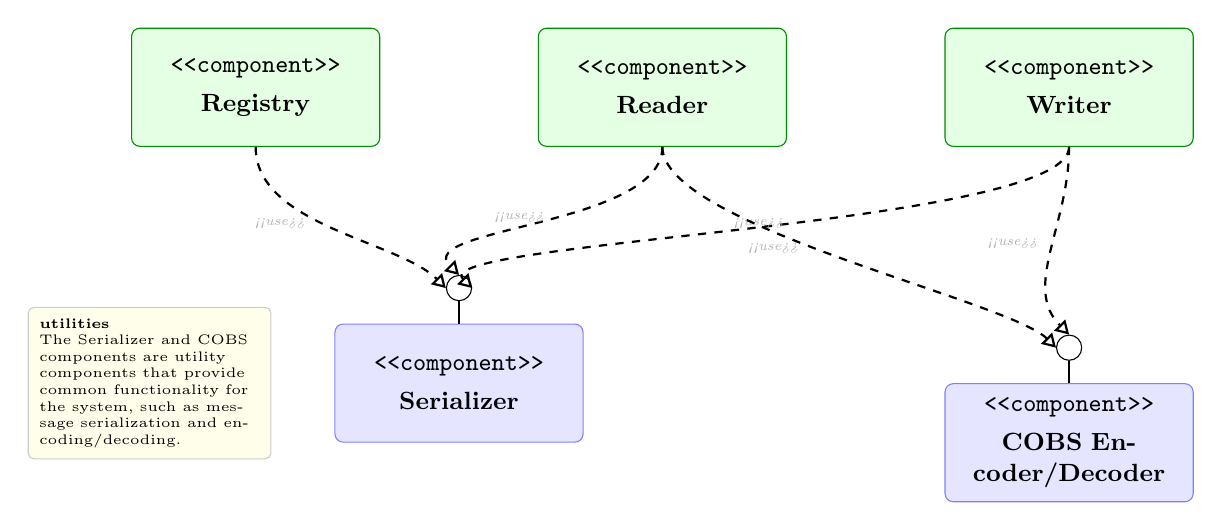
\begin{tikzpicture}[
    % ── node styles ─────────────────────────────────────────
    comp/.style = { draw, rounded corners=3pt, minimum width=3.0cm, minimum
            height=1.5cm, text width=2.8cm, align=center, font=\small, inner sep=5pt, },
    lollipop/.style = { draw, circle, minimum size=0.32cm, inner sep=0pt,
            fill=white, }, stereo/.style = {font=\tiny\itshape, text=gray!60}, use/.style =
    {->, >={Triangle[open]}, dashed, thick}, realize/.style = {->,
    >={Triangle[open]}, dashed, thick, double distance=1.2pt}, assoc/.style =
        {thick}, note/.style = { draw=gray!40, fill=yellow!8, rounded corners=2pt,
            font=\tiny, text width=2.8cm, align=left, inner sep=4pt, }, node distance =
    1.4cm, ]

    % ============================================================
    % ROW 1 — Registry  |  Reader |  Writer
    % ============================================================
    \node[comp, fill=green!10, draw=green!55!black]
    (registry) at (0,0)
    {\texttt{<<component>>}\\[3pt]\textbf{Registry}};

    \node[comp, fill=green!10, draw=green!55!black,
        right=2.0cm of registry]
    (reader)
    {\texttt{<<component>>}\\[3pt]\textbf{Reader}};

    \node[comp, fill=green!10, draw=green!55!black,
        right=2.0cm of reader]
    (writer)
    {\texttt{<<component>>}\\[3pt]\textbf{Writer}};

    % ============================================================
    % ROW 2 — Serializer  |  COBS
    % ============================================================
    \node[comp, fill=blue!10, draw=blue!50,
        below=3.0cm of $(registry)!0.5!(reader)$]
    (serializer)
    {\texttt{<<component>>}\\[3pt]\textbf{Serializer}};
    \node[comp, fill=blue!10, draw=blue!50,
        below=3.0cm of writer]
    (cobs)
    {\texttt{<<component>>}\\[3pt]\textbf{COBS Encoder/Decoder}};

    % ============================================================
    % ROW 3 — DTAPI
    % ============================================================

    % ============================================================
    % ROW 4 — Hardware
    % ============================================================

    % ============================================================
    % PROVIDED INTERFACE LOLLIPOPS
    % ============================================================
    \node[lollipop](serializer-lollipop) at ($(serializer.north)+(0,0.45)$){};
    \node[lollipop](cobs-lollipop) at ($(cobs.north)+(0,0.45)$){};

    \draw[assoc] (serializer.north) -- (serializer-lollipop);
    \draw[assoc] (cobs.north) -- (cobs-lollipop);

    % ============================================================
    % DEPENDENCY ARROWS
    % ============================================================
    % Registry --<<use>>--> Serializer
    \draw[use]
    (registry.south) .. controls +(0,-1.0) and +(-0.6, 0.6) .. (serializer-lollipop.west)
    node[stereo, pos=0.45, left=2pt] {<<use>>};
    \draw[use]
    (reader.south) .. controls +(0,-1.0) and +(-0.6, 0.6) .. (serializer-lollipop.north)
    node[stereo, pos=0.45, left=2pt] {<<use>>};
    \draw[use]
    (writer.south) .. controls +(0,-1.0) and +(-0.6, 0.6) .. (serializer-lollipop.east)
    node[stereo, pos=0.45, left=2pt] {<<use>>};

    \draw[use]
    (reader.south) .. controls +(0,-1.0) and +(-0.6, 0.6) .. (cobs-lollipop.west)
    node[stereo, pos=0.45, left=2pt] {<<use>>};
    \draw[use]
    (writer.south) .. controls +(0,-1.0) and +(-0.6, 0.6) .. (cobs-lollipop.north)
    node[stereo, pos=0.45, left=2pt] {<<use>>};

    % ============================================================
    % ANNOTATION NOTE
    % ============================================================
    \node[note, left=0.8cm of serializer] (note-utility) {
        \textbf{utilities}\\
        The Serializer and COBS components are utility components that provide
        common functionality for the system, such as message serialization and
        encoding/decoding.
    };

\end{tikzpicture}